\chapter{语言模型}
    语言模型可以分为文法型模型和统计语言模型。在实际应用中语言识别、手写体文字识别、机器翻译、键盘输入、信息检索等研究领域都用到了语言模型。文法型语言模型是人工编制的语言学文法,文法规则来源于语言学家掌握的语言学知识和领域知识,但这种语言模型不能处理大规模真实文本。因此,统计语言模型出现了,并且得到了广泛的应用,统计语言模型是基于概率的,包括了N元文法模型(N-gram Model)、隐马尔科夫模型(Hidden Markov Model,简称HMM)、最大熵模型(Maximum Entropy Model)。

    \section{统计语言模型的基本原理}

    统计语言模型是以概率分布的形式说明了一个字符串出现的概率。
    假设词(word)是语言的最小单位,
    句子S是由一系列的词$w_1,w_2, \dots,w_k$顺序构成,
    则句子S的概率为下:
    \begin{equation}
        \begin{split}
            p(s) &= p(w_1)p(w_2|w_1)\dots p(w_n|w_1,w_2,\dots,w_{n-1}) \\
            &=\prod_{i=1}^{n}p(w_i|w_1,w_2,\dots,w_{i-1}) 
        \end{split}
    \end{equation}

    且,上式中约定$p(w_1|w_0)=p(w_1)$.观察上式可以发现,句子S的概率计算是很复杂的,因此,往往采用一些方法来估计语料库中句子的概率。

    \section{主要的统计语言模型}
    \subsection{上下文无关模型}
    上下文无关模型就是词$w_1$的出现与它所处的环境无关,仅仅是它在语料中出现的概率,即它是n-gram中n=1的情况,但是实际上,这种方法效果并不是很好。

    \subsection{n-gram模型}
    n-gram模型是要考虑上下文的。$w_1$出现的是依赖于它之前的n-1个词的,即需要计算词表中的每一个n-1元组的概率,此计算量是巨大的,因此实际中,常取n=2 或n=3.

    \chapter{Hierarchical Softmax模型}
    \section{词向量}
    词向量目前常用的有2种表示方法,One-hot representation 
    和 distributed representation. 词向量,
    顾名思义就是将一个词表示为向量的形式,一个词,
    怎么可以将其表现为向量呢?最简单的就是
    \textbf{One-hot representation},
    它是以词典V中的词的个数作为向量的维度,
    按照字典序或某种特定的顺序将V排序后,
    词w的向量可以表示为: $[0, 0, 1, 0, 0 , \dots, 0]$,
    即词w出现的位置为1,其余均为0. 可以看到,
    这种方法表示的词向量太过于稀疏,维度太高,会引起维度灾难,
    而且非常不利于计算词之间的相似度。另一种\textbf{distributed representation}
    可以解决上述问题,它通过训练将一个词映射为相对于
    One-hot representation来说一个比较短的向量,它的表示形式类似于:
    [0.1,0.34,0.673,0.983]。词向量就是将词映射到词典空间中,
    如下图所示的词向量是两种不同的语言映射。

    \begin{figure}[h]
        \begin{center}
            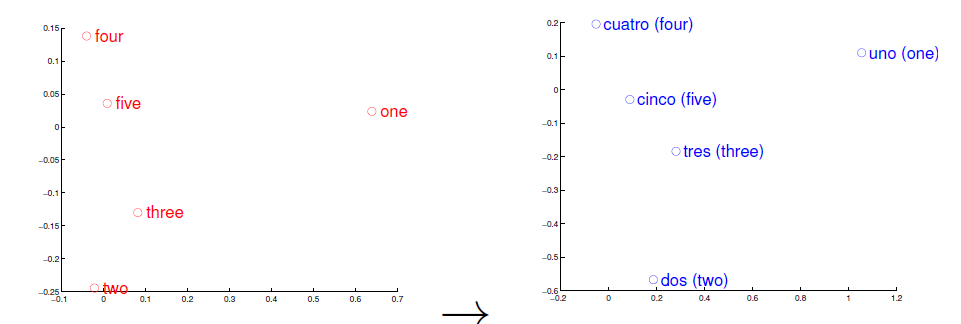
\includegraphics[width=13cm,height=5cm]{2_1}
            \caption{词向量在空间中的映射}
        \end{center}
    \end{figure}

    \section{CBOW模型}
    \subsection{CBOW模型介绍}
    CBOW模型很像 feedforward NNLM(\href{http://jmlr.org/papers/volume3/bengio03a/bengio03a.pdf}{A Neural Probabilistic Language Model}),
    feedforward NNLM模型如下所示:
    \begin{figure}[h]
        \begin{center}
            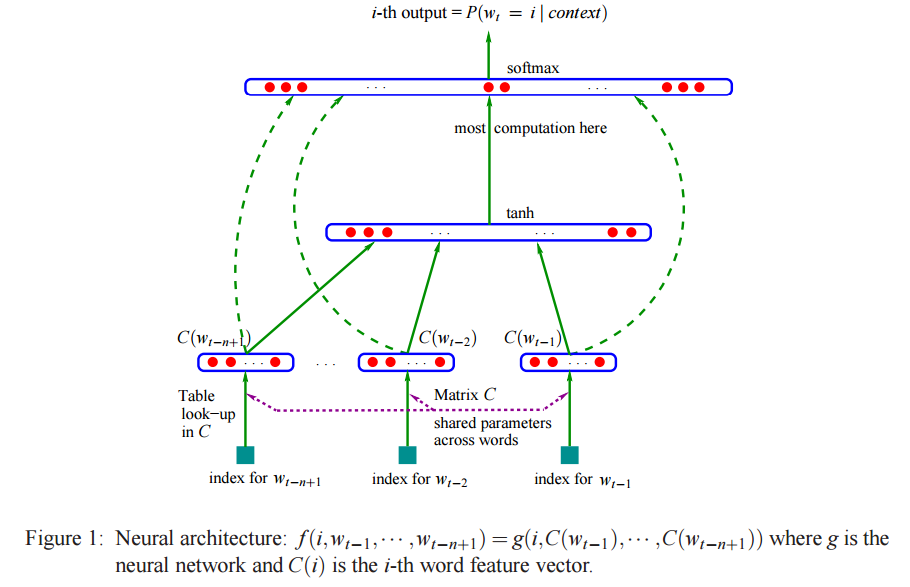
\includegraphics[width=13cm,height=8cm]{2_2}
            \caption{feedforward NNLM模型}
        \end{center}
    \end{figure}

    其中C是一个词向量矩阵,首先,将词$w_i$的词向量从C中取出,
    并且首尾相接组成$\boldsymbol{x}$作为神经网络的第一层输入层,第二层为隐藏层,
    通过 $d+Hx$ 计算得到。$d$ 是一个偏置项。在此之后,使用 $\tanh$ 作为激活函。
    第三层输出层,一共有 $|V|$ 个节点,每个节点 $y_i$ 表示下一个词为$i$的未归一化 
    log 概率。最后使用 softmax 激活函数将输出值 
    $y$ 归一化成概率。最终,$y$ 的计算公式为:$y = b + Wx + U\tanh(d+Hx)$。


    CBOW将隐藏层移除,投影层不再是词向量的拼接,而是各个词向量相加后取平均作为输入,
    由上图可以看到,NNLM模型大部分的计算量在输出层上的softmax归一化运算,
    因此,CBOW为了简化模型,在输出层输出huffman树。CBOW模型根据上下文预测当前词。
    Skip-gram模型是用每个当前词去预测一定范围内除当前词之外前后的词。
    并不是有些人说的CBOW的相反版本。论文关于这一点的原文是:
    \textbf{we use each current word as an input to a log-linear classifier with continuous projection layer, and predict words within a certain range before and after the current word.} 
    \href{http://arxiv.org/pdf/1301.3781v3.pdf}{原文pdf}

    \begin{figure}[h]
        \begin{center}
            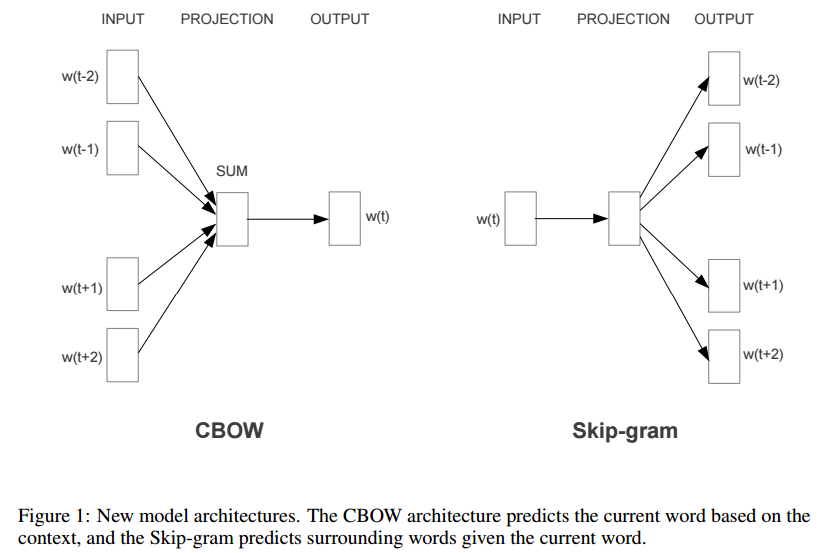
\includegraphics[width=12cm,height=8cm]{2_3}
            \caption{CBOW模型和Skip-gram模型}
        \end{center}
    \end{figure}

    \subsection{CBOW模型的推导}
    由于模型的输出是一颗huffman树,其中树的叶子节点表示词,
    根节点表示权值。
    CBOW的核心内容是推导出$p(w|context(w))$,其中,$context(w)$由w前后各c个词组成。
    如下图所示:下图借用
    \href{http://blog.csdn.net/itplus/article/details/37969979}{基于 Hierarchical Softmax 的模型}.

    \begin{figure}[h]
        \begin{center}
            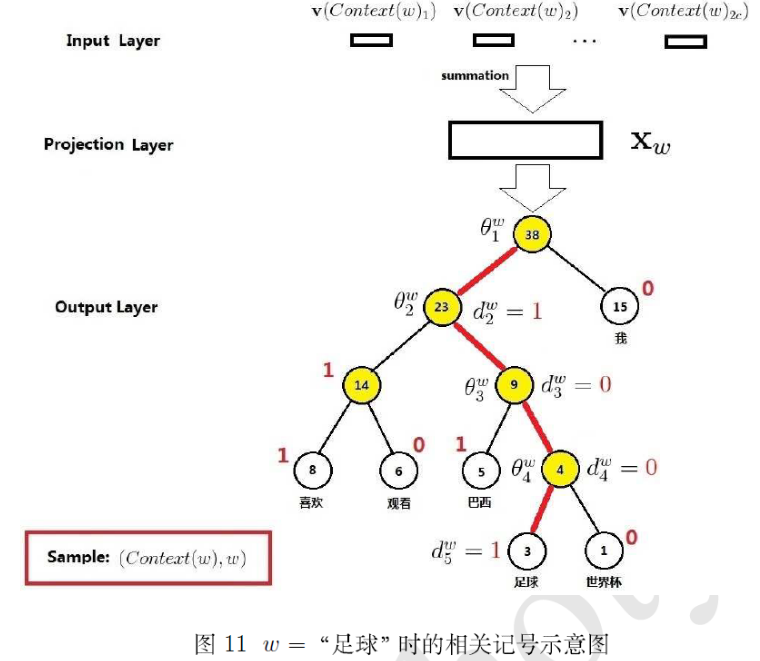
\includegraphics[width=12cm,height=13cm]{2_4}
            \caption{CBOW模型示意图}
        \end{center}
    \end{figure}

    \begin{enumerate}
        \item 由输入层$context(w)$得到投影层向量$\boldsymbol{X_w}$:
        \begin{equation}
            \boldsymbol{X_w} = \sum_{i=1}^{2c} \boldsymbol{V}(context(w)_i)
        \end{equation}
        以上$\boldsymbol{V}(context(w)_i)$初始化为$[\frac{-0.5}{M},\frac{0.5}{M}]$,M为向量的维数。
        \item 由huffman树的根节点到叶节点,是多个二分类问题。二分类问题一般用logistic回归解决,给出回归函数:
        \begin{equation}
            \sigma(z_i) = \frac{1}{1+e^{-z_i}},
        \end{equation} 
        其中,$z=\boldsymbol{X_w^T\theta}$, 
        则
        \begin{equation}
            \Bigg\{ 
                \begin{array} {ll}
                    p(d_i^w|\boldsymbol{X_w^T;\theta_{i-1}})=1-\sigma(z) &, d=1\\
                    p(d_i^w|\boldsymbol{X_w^T;\theta_{i-1}})=\sigma(z) &, d=0
                \end{array}
        \end{equation}

        \item 由以上huffman树的图可知:
        \begin{equation}
            p(w|context(w))=\prod_{i=2}^{l^w} p(d_i^w|\boldsymbol{X_w;\theta_{i-1}})=\prod_{i=2}^{l^w}[\sigma(z_{i-1})^{1-d_i^w}(1-\sigma(z_{i-1}))^{d_i^w}]
        \end{equation}
        \item 语言模型的目标函数是取如下最大似然函数
        \begin{equation}
            \begin{split}
                \mathcal{L}&=\sum_{w \in  \mathcal{C}} \log p(w|context(w))\\
                &=\sum_{w \in  \mathcal{C}} \log \prod_{i=2}^{l^w}[\sigma(z_{i-1})^{1-d_i^w}(1-\sigma(z_{i-1}))^{d_i}]\\
                &=\sum_{w \in  \mathcal{C}}\sum_{i=2}^{l^w}[(1-d_i^w)\log\sigma(z_{i-1})+d_i^w \log (1-\sigma(z_{i-1}))]
            \end{split}
        \end{equation}
        记以下函数为:
        \begin{equation}
            \mathcal{L}(w, i) = (1-d_i^w)\log\sigma(z_{i-1})+d_i^w \log (1-\sigma(z_{i-1})) \\
        \end{equation}
        将$z_i$代入得:
        \begin{equation}
            \mathcal{L}(w, i) = (1-d_i^w)\log\sigma(\boldsymbol{X_w^T\theta_{i-1}})+d_i^w \log (1-\sigma(\boldsymbol{X_w^T\theta_{i-1}})
        \end{equation}
        
        \item 求函数$\mathcal{L}(w, i)$对$w$和$\theta_{i-1}$求偏导数:
        \begin{equation}
            \frac{\partial \mathcal{L}(w, i)}{\partial \boldsymbol{X_w}} = (1-d_i^w-\frac{1}{1+e^{\boldsymbol{-X_w^T\theta_i-1}}})\boldsymbol{\theta_{i-1}}
        \end{equation}
        \begin{equation}
            \frac{\partial \mathcal{L}(w, i)}{\partial \boldsymbol{\theta_{i-1}}} = (1-d_i^w-\frac{1}{1+e^{\boldsymbol{-X_w^T\theta_i-1}}})\boldsymbol{X_w^T}
        \end{equation}

        \item 那么,参数$\theta_{i-1}$的更新公式如下所示:
        \begin{equation}
            \theta_{i-1} := \theta_{i-1} + \eta (1-d_i^w-\frac{1}{1+e^{\boldsymbol{-X_w^T\theta_i-1}}})\boldsymbol{X_w^T}
        \end{equation}
        我们的目的是求每个词的词向量,那么,给出词向量的更新公式:对于每个$w \in context(w)$,都有:
        \begin{equation}
            v(w):=v(w)+\eta \sum_{i=2}^{l_w}(1-d_i^w-\frac{1}{1+e^{\boldsymbol{-X_w^T\theta_i-1}}})\boldsymbol{\theta_{i-1}}
        \end{equation}
    \end{enumerate}

    \section{Skip-gram模型}
    \subsection{Skip-gram模型介绍}
    Skip-gram模型并不是和CBOW模型相反的,
    它们的目的都是计算出词的向量,只不过在作者的论文中给出的图看样子是反的而已。
    Skip-gram模型是用每个当前词去预测一定范围内除当前词之外前后的词。
    同样的,此模型也是输出一颗huffman树,如下图所示:
    \begin{figure}[h]
        \begin{center}
            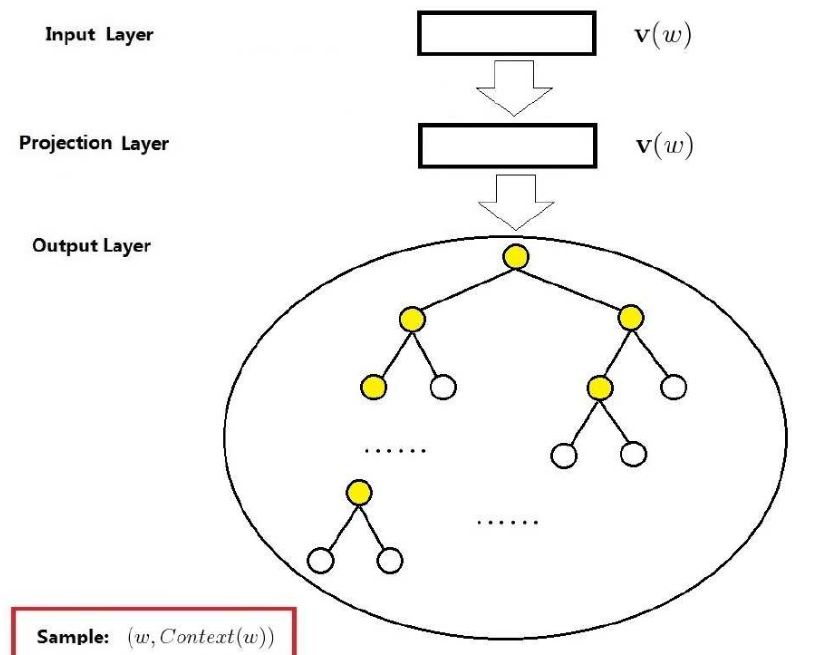
\includegraphics[width=12cm,height=13cm]{3_1}
            \caption{huffman树}
        \end{center}
    \end{figure}
    此图也借用下图借用 
    \href{http://blog.csdn.net/itplus/article/details/37969979}{基于 Hierarchical Softmax 的模型}

    \subsection{Skip-gram模型的目标函数}
    由于Skip-gram的模型输入是当前词,目的是预测它周围的词,因此,此任务的目标函数如下所示:
    \begin{equation}
        \mathcal{L} = \sum_{w \in C} \log P(context(w)|w)
    \end{equation}

    由于$context(w)$ 是一个句子,因此,可以将$P(context(w)|w)$写成如下形式:
    \begin{equation}
        P(context(w)|w) = \prod_{u \in context(w)}P(u|w)
    \end{equation}
    根据hierarchical softmax的讨论:
    \begin{equation}
        P(u|w) = \prod_{j=2}^{l^u}P(d_j^u|v(u); \theta_{j-1})
    \end{equation}
    那么:最终的目标函数可以写为:
    \begin{equation}
        \mathcal{L} = \sum_{w \in C} \log \prod_{u \in context(w)} \prod_{j=2}^{l^u}P(d_j^w|v(u); \theta_{j-1})
    \end{equation}

    \subsection{Skip-gram模型的推导过程}
    \begin{equation}
        \begin{split}
            \mathcal{L} &= \sum_{w \in C} \log \prod_{u \in context(w)} \prod_{j=2}^{l^u}P(d_j^w|v(u); \theta_{j-1}) \\
            &= \sum_{w \in C}\sum_{u \in context(w)} \sum_{j=2}^{l^u} \log P(d_j^w|v(u); \theta_{j-1})\\
            &= \sum_{w \in C}\sum_{u \in context(w)} \sum_{j=2}^{l^u} \log \{ [1-\sigma(v(w)^T\theta_{j-1}^{u})]^{d_j^u} \sigma(v(w)^T\theta_{j-1}^{u})]^{1-d_j^u} \}\\
            &=\sum_{w \in C}\sum_{u \in context(w)} \sum_{j=2}^{l^u} \{d_j^u\log [1-\sigma(v(w)^T\theta_{j-1}^{u})] + (1-d_j^u)\log [\sigma(v(w)^T\theta_{j-1}^{u})]\}
        \end{split}
    \end{equation}

    令
    \begin{equation}
        f = d_j^u\log [1-\sigma(v(w)^T\theta_{j-1}^{u})] + (1-d_j^u)\log [\sigma(v(w)^T\theta_{j-1}^{u})]
    \end{equation}
    则分别求出$f$对$\theta_j$ 和$v(w)$求偏导数:
    \begin{equation}
        \frac{\partial{f}}{\partial{\theta_{j-1}^{u}}}=[1-d_j^u-\sigma(v(w)^T\theta_{j-1}^{u})] v(w)
    \end{equation}
    \begin{equation}
        \frac{\partial{f}}{\partial{v(w)}} = [1-d_j^u-\sigma(v(w)^T\theta_{j-1}^{u})] \theta_{j-1}^{u}
    \end{equation}

    那么$\theta$和$v(w)$的更新公式如下:
    \begin{equation}
        \theta_{j-1}^{u} :=\theta_{j-1}^{u}+\eta [1-d_j^u-\sigma(v(w)^T\theta_{j-1}^{u})] v(w)
    \end{equation}
    \begin{equation}
        v(w):=v(w)+\sum_{u \in context(w)} \sum_{j=2}^{l^u}[1-d_j^u-\sigma(v(w)^T\theta_{j-1}^{u})] \theta_{j-1}^{u}
    \end{equation}




